%% bare_jrnl.tex
%% V1.3
%% 2007/01/11
%% by Michael Shell
%% see http://www.michaelshell.org/
%% for current contact information.
%%
%% This is a skeleton file demonstrating the use of IEEEtran.cls
%% (requires IEEEtran.cls version 1.7 or later) with an IEEE journal paper.
%%
%% Support sites:
%% http://www.michaelshell.org/tex/ieeetran/
%% http://www.ctan.org/tex-archive/macros/latex/contrib/IEEEtran/
%% and
%% http://www.ieee.org/

%HELLO WORLD!


% *** Authors should verify (and, if needed, correct) their LaTeX system  ***
% *** with the testflow diagnostic prior to trusting their LaTeX platform ***
% *** with production work. IEEE's font choices can trigger bugs that do  ***
% *** not appear when using other class files.                            ***
% The testflow support page is at:
% http://www.michaelshell.org/tex/testflow/


%%*************************************************************************
%% Legal Notice:
%% This code is offered as-is without any warranty either expressed or
%% implied; without even the implied warranty of MERCHANTABILITY or
%% FITNESS FOR A PARTICULAR PURPOSE! 
%% User assumes all risk.
%% In no event shall IEEE or any contributor to this code be liable for
%% any damages or losses, including, but not limited to, incidental,
%% consequential, or any other damages, resulting from the use or misuse
%% of any information contained here.
%%
%% All comments are the opinions of their respective authors and are not
%% necessarily endorsed by the IEEE.
%%
%% This work is distributed under the LaTeX Project Public License (LPPL)
%% ( http://www.latex-project.org/ ) version 1.3, and may be freely used,
%% distributed and modified. A copy of the LPPL, version 1.3, is included
%% in the base LaTeX documentation of all distributions of LaTeX released
%% 2003/12/01 or later.
%% Retain all contribution notices and credits.
%% ** Modified files should be clearly indicated as such, including  **
%% ** renaming them and changing author support contact information. **
%%
%% File list of work: IEEEtran.cls, IEEEtran_HOWTO.pdf, bare_adv.tex,
%%                    bare_conf.tex, bare_jrnl.tex, bare_jrnl_compsoc.tex
%%*************************************************************************

% Note that the a4paper option is mainly intended so that authors in
% countries using A4 can easily print to A4 and see how their papers will
% look in print - the typesetting of the document will not typically be
% affected with changes in paper size (but the bottom and side margins will).
% Use the testflow package mentioned above to verify correct handling of
% both paper sizes by the user's LaTeX system.
%
% Also note that the "draftcls" or "draftclsnofoot", not "draft", option
% should be used if it is desired that the figures are to be displayed in
% draft mode.
%
\documentclass[journal,a4paper]{IEEEtran}
%
% If IEEEtran.cls has not been installed into the LaTeX system files,
% manually specify the path to it like:
 %\documentclass[journal]{../sty/IEEEtran}


\usepackage[utf8]{inputenc}

\usepackage{color}
\usepackage{float}


% Some very useful LaTeX packages include:
% (uncomment the ones you want to load)


% *** MISC UTILITY PACKAGES ***
%
%\usepackage{ifpdf}
% Heiko Oberdiek's ifpdf.sty is very useful if you need conditional
% compilation based on whether the output is pdf or dvi.
% usage:
% \ifpdf
%   % pdf code
% \else
%   % dvi code
% \fi
% The latest version of ifpdf.sty can be obtained from:
% http://www.ctan.org/tex-archive/macros/latex/contrib/oberdiek/
% Also, note that IEEEtran.cls V1.7 and later provides a builtin 
% \ifCLASSINFOpdf conditional that works the same way.
% When switching from latex to pdflatex and vice-versa, the compiler may
% have to be run twice to clear warning/error messages.






% *** CITATION PACKAGES ***
%
%\usepackage{cite}
% cite.sty was written by Donald Arseneau
% V1.6 and later of IEEEtran pre-defines the format of the cite.sty package
% \cite{} output to follow that of IEEE. Loading the cite package will
% result in citation numbers being automatically sorted and properly
% "compressed/ranged". e.g., [1], [9], [2], [7], [5], [6] without using
% cite.sty will become [1], [2], [5]--[7], [9] using cite.sty. cite.sty's
% \cite will automatically add leading space, if needed. Use cite.sty's
% noadjust option (cite.sty V3.8 and later) if you want to turn this off.
% cite.sty is already installed on most LaTeX systems. Be sure and use
% version 4.0 (2003-05-27) and later if using hyperref.sty. cite.sty does
% not currently provide for hyperlinked citations.
% The latest version can be obtained at:
% http://www.ctan.org/tex-archive/macros/latex/contrib/cite/
% The documentation is contained in the cite.sty file itself.






% *** GRAPHICS RELATED PACKAGES ***
%
\ifCLASSINFOpdf
\usepackage[pdftex]{graphicx}
  % declare the path(s) where your graphic files are
  % \graphicspath{{../pdf/}{../jpeg/}}
  % and their extensions so you won't have to specify these with
  % every instance of \includegraphics
  % \DeclareGraphicsExtensions{.pdf,.jpeg,.png}
\else
  % or other class option (dvipsone, dvipdf, if not using dvips). graphicx
  % will default to the driver specified in the system graphics.cfg if no
  % driver is specified.
  % \usepackage[dvips]{graphicx}
  % declare the path(s) where your graphic files are
  % \graphicspath{{../eps/}}
  % and their extensions so you won't have to specify these with
  % every instance of \includegraphics
  % \DeclareGraphicsExtensions{.eps}
\fi
\usepackage{epstopdf}
% graphicx was written by David Carlisle and Sebastian Rahtz. It is
% required if you want graphics, photos, etc. graphicx.sty is already
% installed on most LaTeX systems. The latest version and documentation can
% be obtained at: 
% http://www.ctan.org/tex-archive/macros/latex/required/graphics/
% Another good source of documentation is "Using Imported Graphics in
% LaTeX2e" by Keith Reckdahl which can be found as epslatex.ps or
% epslatex.pdf at: http://www.ctan.org/tex-archive/info/
%
% latex, and pdflatex in dvi mode, support graphics in encapsulated
% postscript (.eps) format. pdflatex in pdf mode supports graphics
% in .pdf, .jpeg, .png and .mps (metapost) formats. Users should ensure
% that all non-photo figures use a vector format (.eps, .pdf, .mps) and
% not a bitmapped formats (.jpeg, .png). IEEE frowns on bitmapped formats
% which can result in "jaggedy"/blurry rendering of lines and letters as
% well as large increases in file sizes.
%
% You can find documentation about the pdfTeX application at:
% http://www.tug.org/applications/pdftex





% *** MATH PACKAGES ***
%
%\usepackage[cmex10]{amsmath}
% A popular package from the American Mathematical Society that provides
% many useful and powerful commands for dealing with mathematics. If using
% it, be sure to load this package with the cmex10 option to ensure that
% only type 1 fonts will utilized at all point sizes. Without this option,
% it is possible that some math symbols, particularly those within
% footnotes, will be rendered in bitmap form which will result in a
% document that can not be IEEE Xplore compliant!
%
% Also, note that the amsmath package sets \interdisplaylinepenalty to 10000
% thus preventing page breaks from occurring within multiline equations. Use:
%\interdisplaylinepenalty=2500
% after loading amsmath to restore such page breaks as IEEEtran.cls normally
% does. amsmath.sty is already installed on most LaTeX systems. The latest
% version and documentation can be obtained at:
% http://www.ctan.org/tex-archive/macros/latex/required/amslatex/math/





% *** SPECIALIZED LIST PACKAGES ***
%
%\usepackage{algorithmic}
% algorithmic.sty was written by Peter Williams and Rogerio Brito.
% This package provides an algorithmic environment fo describing algorithms.
% You can use the algorithmic environment in-text or within a figure
% environment to provide for a floating algorithm. Do NOT use the algorithm
% floating environment provided by algorithm.sty (by the same authors) or
% algorithm2e.sty (by Christophe Fiorio) as IEEE does not use dedicated
% algorithm float types and packages that provide these will not provide
% correct IEEE style captions. The latest version and documentation of
% algorithmic.sty can be obtained at:
% http://www.ctan.org/tex-archive/macros/latex/contrib/algorithms/
% There is also a support site at:
% http://algorithms.berlios.de/index.html
% Also of interest may be the (relatively newer and more customizable)
% algorithmicx.sty package by Szasz Janos:
% http://www.ctan.org/tex-archive/macros/latex/contrib/algorithmicx/




% *** ALIGNMENT PACKAGES ***
%
%\usepackage{array}
% Frank Mittelbach's and David Carlisle's array.sty patches and improves
% the standard LaTeX2e array and tabular environments to provide better
% appearance and additional user controls. As the default LaTeX2e table
% generation code is lacking to the point of almost being broken with
% respect to the quality of the end results, all users are strongly
% advised to use an enhanced (at the very least that provided by array.sty)
% set of table tools. array.sty is already installed on most systems. The
% latest version and documentation can be obtained at:
% http://www.ctan.org/tex-archive/macros/latex/required/tools/


%\usepackage{mdwmath}
%\usepackage{mdwtab}
% Also highly recommended is Mark Wooding's extremely powerful MDW tools,
% especially mdwmath.sty and mdwtab.sty which are used to format equations
% and tables, respectively. The MDWtools set is already installed on most
% LaTeX systems. The lastest version and documentation is available at:
% http://www.ctan.org/tex-archive/macros/latex/contrib/mdwtools/


% IEEEtran contains the IEEEeqnarray family of commands that can be used to
% generate multiline equations as well as matrices, tables, etc., of high
% quality.


%\usepackage{eqparbox}
% Also of notable interest is Scott Pakin's eqparbox package for creating
% (automatically sized) equal width boxes - aka "natural width parboxes".
% Available at:
% http://www.ctan.org/tex-archive/macros/latex/contrib/eqparbox/





% *** SUBFIGURE PACKAGES ***
%\usepackage[tight,footnotesize]{subfigure}
% subfigure.sty was written by Steven Douglas Cochran. This package makes it
% easy to put subfigures in your figures. e.g., "Figure 1a and 1b". For IEEE
% work, it is a good idea to load it with the tight package option to reduce
% the amount of white space around the subfigures. subfigure.sty is already
% installed on most LaTeX systems. The latest version and documentation can
% be obtained at:
% http://www.ctan.org/tex-archive/obsolete/macros/latex/contrib/subfigure/
% subfigure.sty has been superceeded by subfig.sty.



%\usepackage[caption=false]{caption}
%\usepackage[font=footnotesize]{subfig}
% subfig.sty, also written by Steven Douglas Cochran, is the modern
% replacement for subfigure.sty. However, subfig.sty requires and
% automatically loads Axel Sommerfeldt's caption.sty which will override
% IEEEtran.cls handling of captions and this will result in nonIEEE style
% figure/table captions. To prevent this problem, be sure and preload
% caption.sty with its "caption=false" package option. This is will preserve
% IEEEtran.cls handing of captions. Version 1.3 (2005/06/28) and later 
% (recommended due to many improvements over 1.2) of subfig.sty supports
% the caption=false option directly:
%\usepackage[caption=false,font=footnotesize]{subfig}
%
% The latest version and documentation can be obtained at:
% http://www.ctan.org/tex-archive/macros/latex/contrib/subfig/
% The latest version and documentation of caption.sty can be obtained at:
% http://www.ctan.org/tex-archive/macros/latex/contrib/caption/




% *** FLOAT PACKAGES ***
%
%\usepackage{fixltx2e}
% fixltx2e, the successor to the earlier fix2col.sty, was written by
% Frank Mittelbach and David Carlisle. This package corrects a few problems
% in the LaTeX2e kernel, the most notable of which is that in current
% LaTeX2e releases, the ordering of single and double column floats is not
% guaranteed to be preserved. Thus, an unpatched LaTeX2e can allow a
% single column figure to be placed prior to an earlier double column
% figure. The latest version and documentation can be found at:
% http://www.ctan.org/tex-archive/macros/latex/base/



%\usepackage{stfloats}
% stfloats.sty was written by Sigitas Tolusis. This package gives LaTeX2e
% the ability to do double column floats at the bottom of the page as well
% as the top. (e.g., "\begin{figure*}[!b]" is not normally possible in
% LaTeX2e). It also provides a command:
%\fnbelowfloat
% to enable the placement of footnotes below bottom floats (the standard
% LaTeX2e kernel puts them above bottom floats). This is an invasive package
% which rewrites many portions of the LaTeX2e float routines. It may not work
% with other packages that modify the LaTeX2e float routines. The latest
% version and documentation can be obtained at:
% http://www.ctan.org/tex-archive/macros/latex/contrib/sttools/
% Documentation is contained in the stfloats.sty comments as well as in the
% presfull.pdf file. Do not use the stfloats baselinefloat ability as IEEE
% does not allow \baselineskip to stretch. Authors submitting work to the
% IEEE should note that IEEE rarely uses double column equations and
% that authors should try to avoid such use. Do not be tempted to use the
% cuted.sty or midfloat.sty packages (also by Sigitas Tolusis) as IEEE does
% not format its papers in such ways.


%\ifCLASSOPTIONcaptionsoff
%  \usepackage[nomarkers]{endfloat}
% \let\MYoriglatexcaption\caption
% \renewcommand{\caption}[2][\relax]{\MYoriglatexcaption[#2]{#2}}
%\fi
% endfloat.sty was written by James Darrell McCauley and Jeff Goldberg.
% This package may be useful when used in conjunction with IEEEtran.cls'
% captionsoff option. Some IEEE journals/societies require that submissions
% have lists of figures/tables at the end of the paper and that
% figures/tables without any captions are placed on a page by themselves at
% the end of the document. If needed, the draftcls IEEEtran class option or
% \CLASSINPUTbaselinestretch interface can be used to increase the line
% spacing as well. Be sure and use the nomarkers option of endfloat to
% prevent endfloat from "marking" where the figures would have been placed
% in the text. The two hack lines of code above are a slight modification of
% that suggested by in the endfloat docs (section 8.3.1) to ensure that
% the full captions always appear in the list of figures/tables - even if
% the user used the short optional argument of \caption[]{}.
% IEEE papers do not typically make use of \caption[]'s optional argument,
% so this should not be an issue. A similar trick can be used to disable
% captions of packages such as subfig.sty that lack options to turn off
% the subcaptions:
% For subfig.sty:
% \let\MYorigsubfloat\subfloat
% \renewcommand{\subfloat}[2][\relax]{\MYorigsubfloat[]{#2}}
% For subfigure.sty:
% \let\MYorigsubfigure\subfigure
% \renewcommand{\subfigure}[2][\relax]{\MYorigsubfigure[]{#2}}
% However, the above trick will not work if both optional arguments of
% the \subfloat/subfig command are used. Furthermore, there needs to be a
% description of each subfigure *somewhere* and endfloat does not add
% subfigure captions to its list of figures. Thus, the best approach is to
% avoid the use of subfigure captions (many IEEE journals avoid them anyway)
% and instead reference/explain all the subfigures within the main caption.
% The latest version of endfloat.sty and its documentation can obtained at:
% http://www.ctan.org/tex-archive/macros/latex/contrib/endfloat/
%
% The IEEEtran \ifCLASSOPTIONcaptionsoff conditional can also be used
% later in the document, say, to conditionally put the References on a 
% page by themselves.





% *** PDF, URL AND HYPERLINK PACKAGES ***
%
%\usepackage{url}
% url.sty was written by Donald Arseneau. It provides better support for
% handling and breaking URLs. url.sty is already installed on most LaTeX
% systems. The latest version can be obtained at:
% http://www.ctan.org/tex-archive/macros/latex/contrib/misc/
% Read the url.sty source comments for usage information. Basically,
% \url{my_url_here}.





% *** Do not adjust lengths that control margins, column widths, etc. ***
% *** Do not use packages that alter fonts (such as pslatex).         ***
% There should be no need to do such things with IEEEtran.cls V1.6 and later.
% (Unless specifically asked to do so by the journal or conference you plan
% to submit to, of course. )


% correct bad hyphenation here
\hyphenation{op-tical net-works semi-conduc-tor}


\begin{document}
%
% paper title
% can use linebreaks \\ within to get better formatting as desired
\title{Development of an experimental setup to perform low-temperature microscopy in a directional magnetic field}
%
%
% author names and IEEE memberships
% note positions of commas and nonbreaking spaces ( ~ ) LaTeX will not break
% a structure at a ~ so this keeps an author's name from being broken across
% two lines.
% use \thanks{} to gain access to the first footnote area
% a separate \thanks must be used for each paragraph as LaTeX2e's \thanks
% was not built to handle multiple paragraphs
%

\author{Molly Bazilchuk, 
David Egger, 
Félix Tora, 
Loïc Schneider}% <-this % stops a space
%\thanks{M. Shell is with the Department
%of Electrical and Computer Engineering, Georgia Institute of Technology, Atlanta,
%GA, 30332 USA e-mail: (see http://www.michaelshell.org/contact.html).}% <-this % stops a space
%\thanks{J. Doe and J. Doe are with Anonymous University.}% <-this % stops a space
%\thanks{Manuscript received April 19, 2005; revised January 11, 2007.}}

% note the % following the last \IEEEmembership and also \thanks - 
% these prevent an unwanted space from occurring between the last author name
% and the end of the author line. i.e., if you had this:
% 
% \author{....lastname \thanks{...} \thanks{...} }
%                     ^------------^------------^----Do not want these spaces!
%
% a space would be appended to the last name and could cause every name on that
% line to be shifted left slightly. This is one of those "LaTeX things". For
% instance, "\textbf{A} \textbf{B}" will typeset as "A B" not "AB". To get
% "AB" then you have to do: "\textbf{A}\textbf{B}"
% \thanks is no different in this regard, so shield the last } of each \thanks
% that ends a line with a % and do not let a space in before the next \thanks.
% Spaces after \IEEEmembership other than the last one are OK (and needed) as
% you are supposed to have spaces between the names. For what it is worth,
% this is a minor point as most people would not even notice if the said evil
% space somehow managed to creep in.



% The paper headers
%\markboth{Journal of \LaTeX\ Class Files,~Vol.~6, No.~1, January~2007}%f
%{Shell \MakeLowercase{\textit{et al.}}: Bare Demo of IEEEtran.cls for Journals}

% The only time the second header will appear is for the odd numbered pages
% after the title page when using the twoside option.
% 
% *** Note that you probably will NOT want to include the author's ***
% *** name in the headers of peer review papers.                   ***
% You can use \ifCLASSOPTIONpeerreview for conditional compilation here if
% you desire.




% If you want to put a publisher's ID mark on the page you can do it like
% this:
%\IEEEpubid{0000--0000/00\$00.00~\copyright~2007 IEEE}
% Remember, if you use this you must call \IEEEpubidadjcol in the second
% column for its text to clear the IEEEpubid mark.



% use for special paper notices
%\IEEEspecialpapernotice{(Invited Paper)}




% make the title area
\maketitle


\begin{abstract}
%\boldmath
 If the temperature of a ferrimagnetic material is raised above the compensation temperature, the material will undergo a transition during which the total magnetic momentum becomes zero. Of particular interest is the development of the magnetic domains in such a material as it undergoes this transition, which can be studied using magneto-optical microscopy. The previous group had fabricated a device which induces a strong vectorial magnetic field on a sample placed inside. Using Labview, we developed a software to control this field. To create the temperature conditions necessary for the compensation point transition to occur, a special cryostat suitable for magneto-optical microscopy was designed to fit inside the magnetic field device. Furthermore, the magnetic field device was tested for interior homogeneity and field strength using a magnetometer. A commercial Toshiba Hall bar was investigated with the goal of making a more precise probe for magnetic field measurements, and electronics were developed to compensate for the internal offset of this device. Our work has created an experimental setup that may be utilized for observation of magnetic transitions, although additional development of the Labview software to accommodate the cryostat is necessary. 
 \end{abstract}
% IEEEtran.cls defaults to using nonbold math in the Abstract.
% This preserves the distinction between vectors and scalars. However,
% if the journal you are submitting to favors bold math in the abstract,
% then you can use LaTeX's standard command \boldmath at the very start
% of the abstract to achieve this. Many IEEE journals frown on math
% in the abstract anyway.

% Note that keywords are not normally used for peerreview papers.
%\begin{IEEEkeywords}
%IEEEtran, journal, \LaTeX, paper, template.
%\end{IEEEkeywords}






% For peer review papers, you can put extra information on the cover
% page as needed:
% \ifCLASSOPTIONpeerreview
% \begin{center} \bfseries EDICS Category: 3-BBND \end{center}
% \fi
%
% For peerreview papers, this IEEEtran command inserts a page break and
% creates the second title. It will be ignored for other modes.
\IEEEpeerreviewmaketitle



\section{Introduction}
% The very first letter is a 2 line initial drop letter followed
% by the rest of the first word in caps.
% form to use if the first word consists of a single letter:
% \IEEEPARstart{A}{demo} file is ....
% form to use if you need the single drop letter followed by
% normal text (unknown if ever used by IEEE):
% \IEEEPARstart{A}{}demo file is ....
% Some journals put the first two words in caps:
% \IEEEPARstart{T}{his demo} file is ....

%\hfill mds
 
%\hfill January 11, 2007

%\subsection{Subsection Heading Here}
%Subsection text here.

% needed in second column of first page if using \IEEEpubid
%\IEEEpubidadjcol

%\subsubsection{Subsubsection Heading Here}
%Subsubsection text here.


% An example of a floating figure using the graphicx package.
% Note that \label must occur AFTER (or within) \caption.
% For figures, \caption should occur after the \includegraphics.
% Note that IEEEtran v1.7 and later has special internal code that
% is designed to preserve the operation of \label within \caption
% even when the captionsoff option is in effect. However, because
% of issues like this, it may be the safest practice to put all your
% \label just after \caption rather than within \caption{}.
%
% Reminder: the "draftcls" or "draftclsnofoot", not "draft", class
% option should be used if it is desired that the figures are to be
% displayed while in draft mode.
%
%\begin{figure}[!t]
%\centering
%\includegraphics[width=2.5in]{myfigure}
% where an .eps filename suffix will be assumed under latex, 
% and a .pdf suffix will be assumed for pdflatex; or what has been declared
% via \DeclareGraphicsExtensions.
%\caption{Simulation Results}
%\label{fig_sim}
%\end{figure}

% Note that IEEE typically puts floats only at the top, even when this
% results in a large percentage of a column being occupied by floats.


% An example of a double column floating figure using two subfigures.
% (The subfig.sty package must be loaded for this to work.)
% The subfigure \label commands are set within each subfloat command, the
% \label for the overall figure must come after \caption.
% \hfil must be used as a separator to get equal spacing.
% The subfigure.sty package works much the same way, except \subfigure is
% used instead of \subfloat.
%
%\begin{figure*}[!t]
%\centerline{\subfloat[Case I]\includegraphics[width=2.5in]{subfigcase1}%
%\label{fig_first_case}}
%\hfil
%\subfloat[Case II]{\includegraphics[width=2.5in]{subfigcase2}%
%\label{fig_second_case}}}
%\caption{Simulation results}
%\label{fig_sim}
%\end{figure*}
%
% Note that often IEEE papers with subfigures do not employ subfigure
% captions (using the optional argument to \subfloat), but instead will
% reference/describe all of them (a), (b), etc., within the main caption.


% An example of a floating table. Note that, for IEEE style tables, the 
% \caption command should come BEFORE the table. Table text will default to
% \footnotesize as IEEE normally uses this smaller font for tables.
% The \label must come after \caption as always.
%
%\begin{table}[!t]
%% increase table row spacing, adjust to taste
%\renewcommand{\arraystretch}{1.3}
% if using array.sty, it might be a good idea to tweak the value of
% \extrarowheight as needed to properly center the text within the cells
%\caption{An Example of a Table}
%\label{table_example}
%\centering
%% Some packages, such as MDW tools, offer better commands for making tables
%% than the plain LaTeX2e tabular which is used here.
%\begin{tabular}{|c||c|}
%\hline
%One & Two\\
%\hline
%Three & Four\\
%\hline
%\end{tabular}
%\end{table}


% Note that IEEE does not put floats in the very first column - or typically
% anywhere on the first page for that matter. Also, in-text middle ("here")
% positioning is not used. Most IEEE journals use top floats exclusively.
% Note that, LaTeX2e, unlike IEEE journals, places footnotes above bottom
% floats. This can be corrected via the \fnbelowfloat command of the
% stfloats package.

\subsection{Magnetism and magneto-optic microscopy}
\IEEEPARstart{A}{ ferrimagnetic} material is one of opposing magnetic moments in different sub lattices. Below the compensation temperature, the sum of these magnetic moments is non-zero and the material is has a net magnetic moment. Above the compensation temperature, the magnetic moments cancel each other out as the material becomes non-magnetic. Yet another transition temperature in such materials is the Curie temperature at which the moments cease to be aligned and instead move randomly. As in \cite{garnet}, we wished to examine the domain development during a transition at the compensation temperature.

The magnetic domains of a sample can be examined graphically using magneto-optic microscopy, either based on Kerr or Faraday effects. Both describe changes in the polarization plane light as it interacts magnetic materials; the Kerr effect describes the changes in light \emph{reflected} from magnetic surfaces with the Faraday effect describes the changes in light \emph{transmitted} through magnetic surfaces. These two effects, along with the correct analyzer filters, allow us to image magnetic domains using an optical microscope.

Our goal was to create an experimental setup combining precise control of strong, directional magnetic fields with a cryostat that allowed temperatures in the range of 100-400K, both of which needed to fit under an optical microscope within the focal length. All of this would ideally be controlled by an intuitive software to allow for easy experiment control.

\subsection{The previous group's work}
Our predecessors had designed and fabricated a device which allowed directional control of a magnetic field of up to 200mT. The device is an 80mm cube made of steel to achieve high permeability. There are 4 sets of opposing coils of copper wired around steel pins through which the field is induced. The coils are designed to precisely focus the magnetic field by their proximity to the sample and their directionality. A model of the cube is displayed in figure \ref{f cube}.

\begin{figure}[h]
\centering
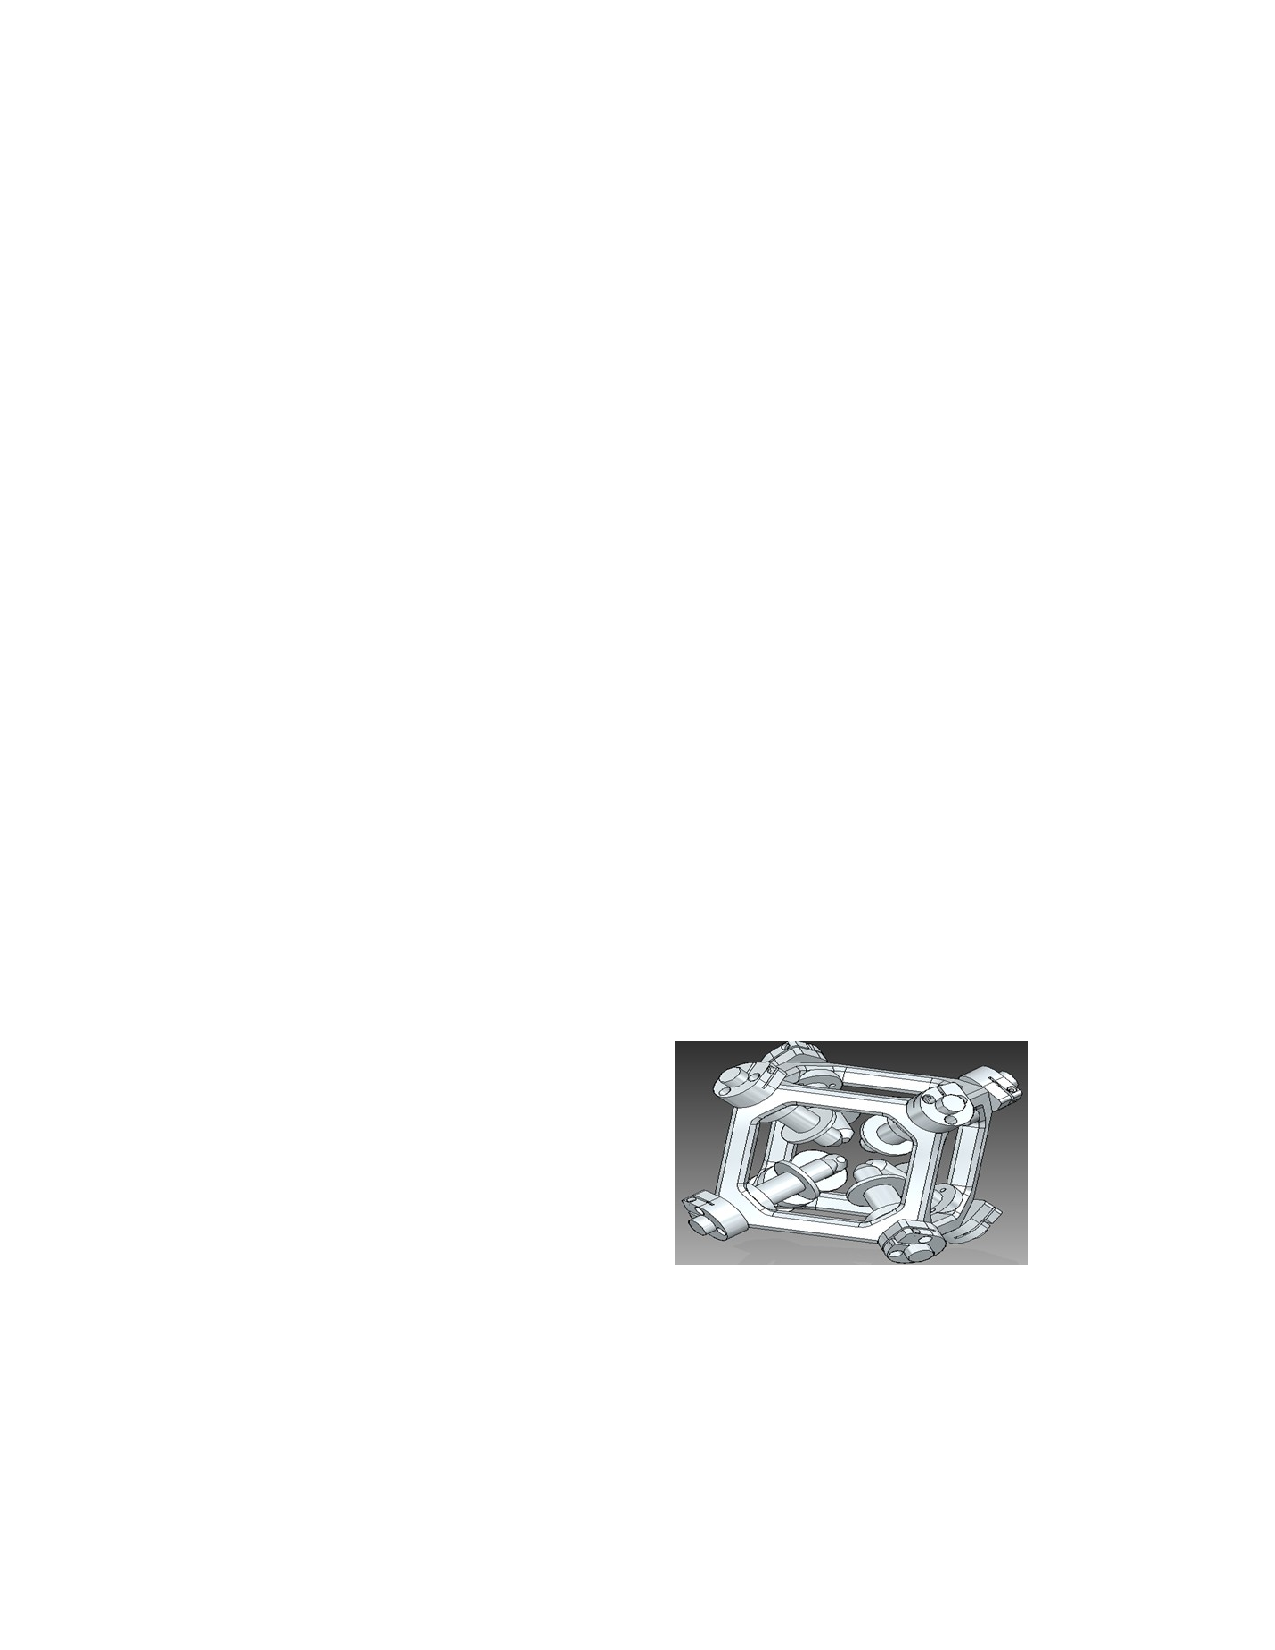
\includegraphics[width=0.45\textwidth,height=0.45 \textwidth]{cube}
\caption{Conceptual image of the field-producing cube designed by the previous group}
\label{f cube}
\end{figure}

\subsection{Objectives}
Building on the previous groups work, our principle objective was to develop a system around the cube that would allow for experiments on ferrimagnetic materials around the compensation temperature. First of all, the cube's magnetic field would need to be characterized for both homogeneity and strength. To this end, it was decided to convert a commercial Hall bar into a gauss meter, in addition to purchasing a standard gauss meter. We believed that with the smaller active area, the Hall bar would provide superior sensing capabilities. Next, a cryostat would need to be built which would allow temperature control between 100K and ambient. This cryostat would of course need to fit inside the cube. Finally, a computer control system would need to be developed to connect the instruments together. The goal was to create a user-friendly software that would allow operators to enter a set of parameters and quickly perform any variety of experiments. An algorithm for directional control of the cube's magnetic field would also have to be developed. 



\section{Conception}
\subsection{Development of the cryostat}
The cryostat needed to be capable of accurately controlling the sample temperature between 100K and ambient, and it also needed to fit in the cube, so as to correctly place the sample in the magnetic field. This last constraint implies that the actual sample chamber should be no larger than a few cubic centimeters. A transparent window above the sample was also needed in order to perform magneto-optical microscopy. The main requirement of this window was that it would not distort the light passing through it, which would disturb the microscopy.

The final design of the cryostat consisted of two parts: the sample holder, and the cooling cavity. These two parts are connected via an exclusively thermal contact. This allows to maintain two separate vacuum levels of different pressure in the two chambers. The sample holder is kept in primary vacuum ($10^-3$ mbar), whereas the cooling cavity is kept in secondary vacuum ($10^-6$ mbar) to improve the thermal isolation in the cooling cavity. Except in case of malfunction, the cooling cavity remains closed so that it will virtually never be pressurized. The vacuum of the sample holder on the other hand needs to be broken frequently in order to change samples. An easier-to-handle and re-establish primary vacuum is preferable in this case, since the main objective of the vacuum in the sample holder is simply to remove residual water molecules.

The interior of the cooling cavity is filled with liquid nitrogen. The nitrogen is topped-off with a tube located at the extremity of the cavity. The nitrogen circles through a series of thin copper cylinders layered on top of each other in the middle of the cavity.  The thermal transfer from the nitrogen to the copper cylinders is maximized by the large surface area of the cylinder. After passing through the cylinders, the nitrogen is removed from the cavity. A model of the cryostat is displayed in figure \ref{f cryostat}.

\begin{figure}[h]
\centering
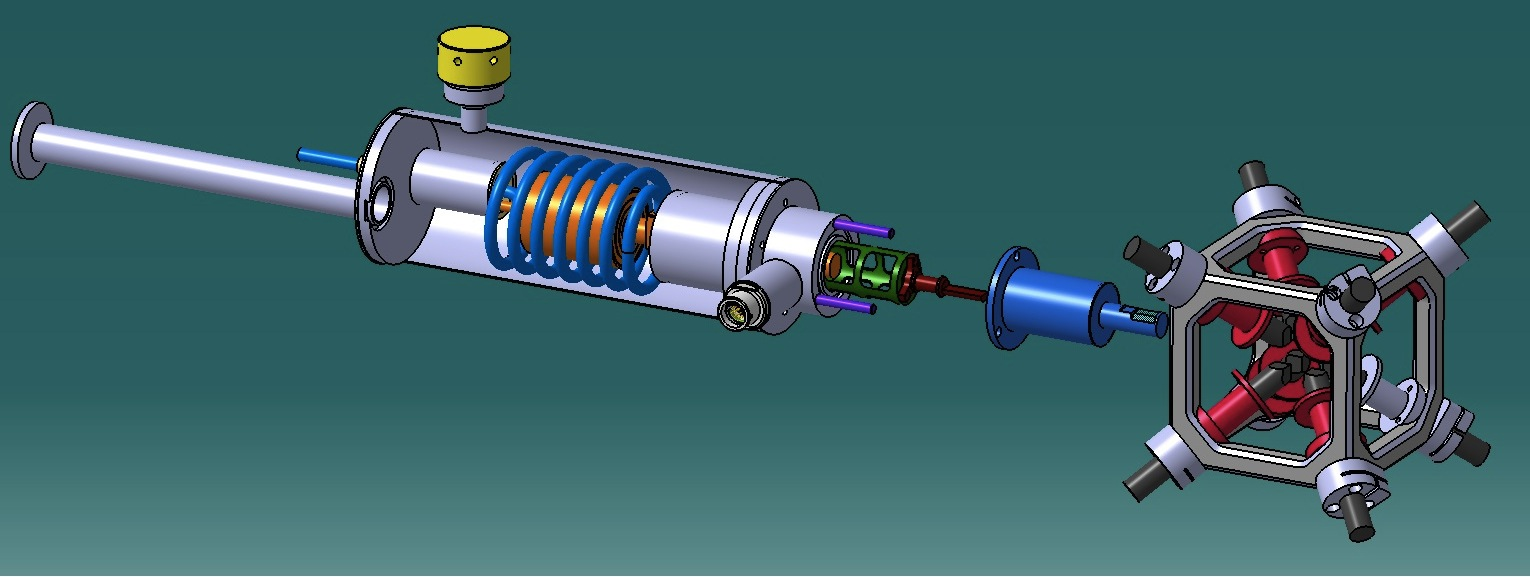
\includegraphics[width=0.45\textwidth]{Cryo_1.jpg}
\caption{Interior view of the cryostat, with the field-producing cube on the right for scale}
\label{f cryostat}
\end{figure}

Inside the sample holder, the sample is placed on a copper finger which has thermal contact to the wired copper tubes in the cooling chamber. A portal made of glass covers the sample. The cover is made of stainless steel, which was chosen for its superior mechanical properties, thermal isolation and the fact that it can be shaped in a thin pieces. A copper wire is wrapped around the extremity of the finger. By sending a current through this wire, the temperature can be regulated. The minimum theoretical temperature is therefore that of liquid nitrogen, 77K. Taking into consideration thermal loses, we hope the cryostat will be able to attain 100K.

An external valve permits maintenance of the interior vacuum. It also doubles as a security measure. If the pressure in the chamber for any reason becomes too high, the valve will open and release the pressure. The design allows pumping nitrogen into the cavity with the same pump that is used to create the vacuum.

\subsection{Development of control software}

Using a computer equipped with both an analog PCI-bus input and output card from ADVANTECH (input: PCI-1715U, output: PCI-1723), we created a Labview program to interactively control the magnetic field in the cube from the computer.

The 4 pairs of copper coils were supplied by a KEPCO bipolar operational amplifier and a custom-made current generator. Both generators were controlled by an external voltage via the Labview program, using the output card as the gateway between program and generator.

\begin{figure}[H]
\centering
\includegraphics[width=0.45\textwidth]{cube_pic}
\caption{The cube as connected to the experimental setup}
\end{figure}

The two independently adjustable current sources allowed a variation of the direction of the generated magnetic field in one or two dimensions. A third independent source would be needed to be able to control the magnetic field in three dimensions. A transfer matrix was calculated to translate from cartesian coordinates (input) to the cube's coordinate system (see appendix \ref{sec:app} for details). The presence of 4 basis vectors in the cube's space implies a linear interdependence  since only three vectors are necessary to span a three-dimensional space. This results in one degree of freedom when applying a current to the cube, which means that there are an infinite number of combinations of input current to give the same output field. The wiring setup of the cube's coils therefore depends on the nature of the experiment performed.
 

\subsection{The Hall bar sensor}
A commercial cross-shaped Hall bar THS118 from Toshiba was chosen to develop the Hall bar magnetic field sensor. This type has already proven to be useful for measuring magnetization in \cite{nishioka}. Due to imperfections in the Hall bar, control electronics needed to be created to obtain accurate measurements. 

\begin{figure}[H]
\centering
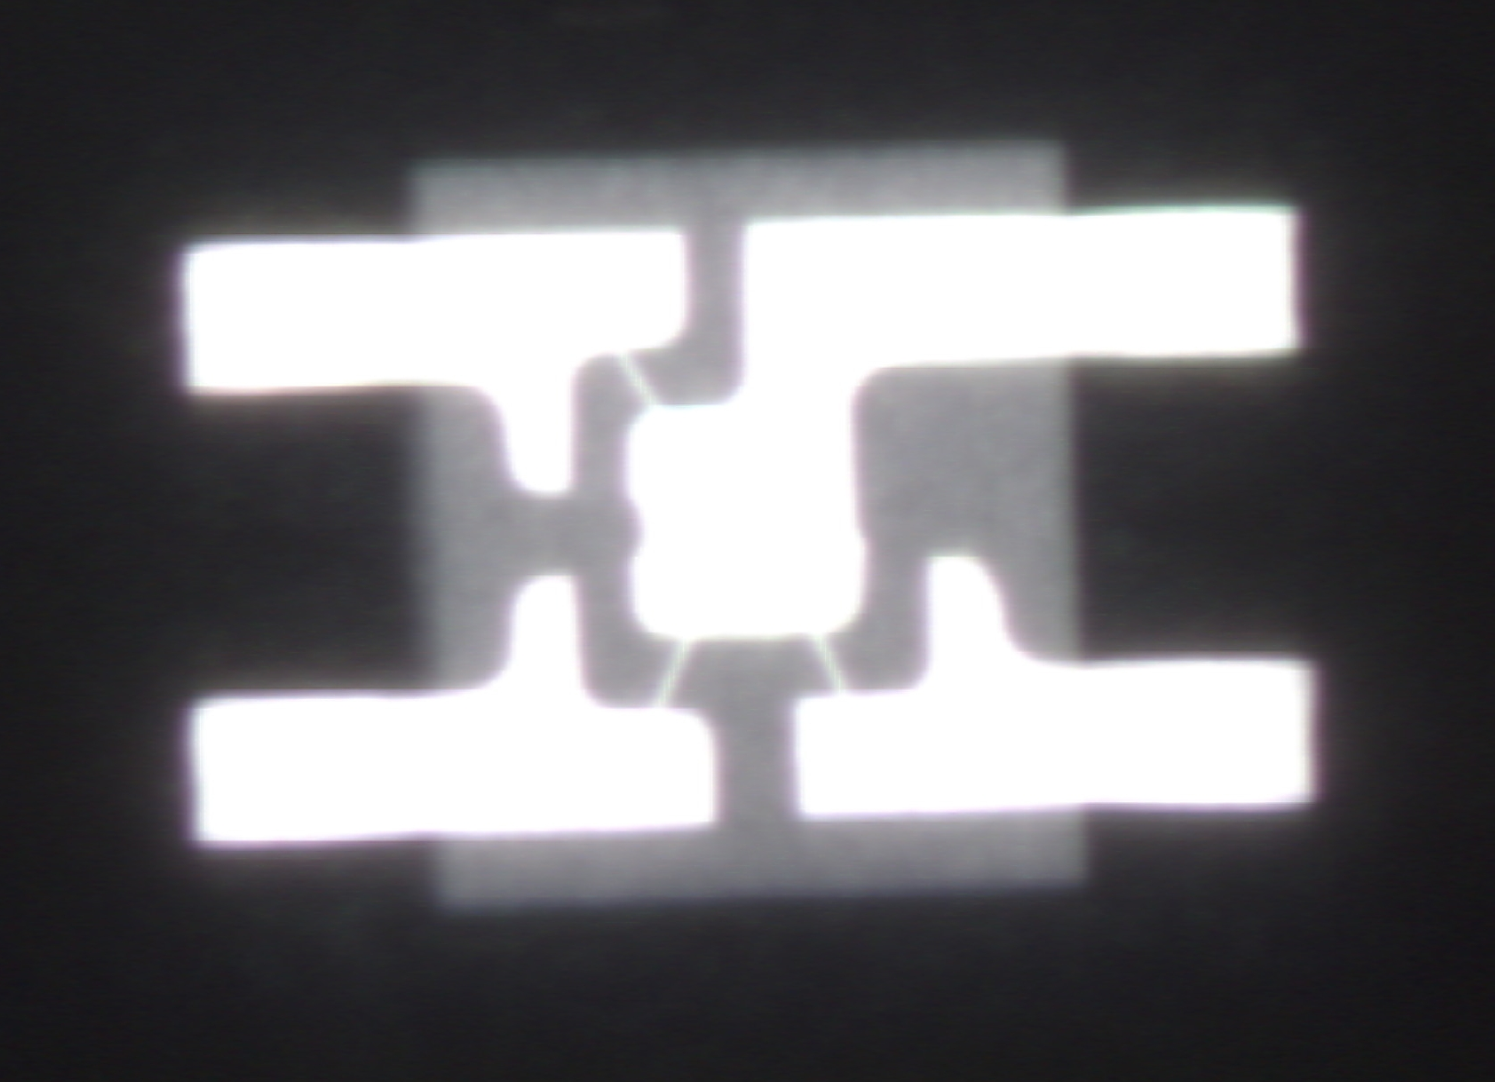
\includegraphics[width=0.45\textwidth]{hallbar}
\caption{An x-ray photograph of the interior of the Toshiba Hall bar}
\end{figure}

As we can see in the image above, the Hall bar is cross-shaped, but not symmetrically so. The measured Hall voltage will depend on the permutation of ends measured upon, so that a different voltage will be obtained in the same magnetic field if ends 1 and 3 are used as opposed to 2-4.

The van der Pauw method \cite{pauw} is crucial in eliminating these geometry-based effects. A spinning current device \cite{steiner} constantly per mutates the pair contacts measuring the Hall voltage and the pair where the current is applied. A continuous variation of the configuration, and averaging over the values, allows to obtain measure of the magnetic field with the effects of geometric asymmetries removed. To this end, a spinning current circuit was fabricated to be used in conjunction with the Hall bar.

The electronic circuit took a sine wave as input, and used a comparator to detect the point at which the sine wave passes zero. A flip-flop switch connected to the comparator was flipped based on the output. Further switches permute the connection of Hall bar contacts(i.e. which ends were connected to the current and which were measured). The frequency of the input sine wave determined the frequency at which the contact pairs are switched around. The sine signal also acts as a current source for the Hall bar. 

\begin{figure}[H]
\centering
\includegraphics[width=0.45\textwidth]{circuit}
\caption{The complete the circuit}
\end{figure}

The circuit was designed and fabricated, but unfortunately was never fully operational. As seen in the Hubble telescope in 1991, small mistakes can propagate and render a system unusable \cite{hubble}. In this case, a mislabeling of a component which served to convert a 10V into a 2.5V output lead to 10V being applied to the entire circuit. As many of the components were not rated for such a high voltage, they were destroyed. Limited time prohibited us from rectifying this error.

\section{Characterization}

\subsection{Experiments}


\subsubsection{On the Hall bar sensor}
The Hall bar sensor is a product designed by Toshiba. The Toshiba data sheet \cite{toshiba} gave us an idea of the properties of the Hall bar. Our goal is to use the hall bar to perform magnetic field measures in the cube, and thus more specific a characterization of its behavior and calibration were necessary. Keeping in mind that the Hall sensor is meant to work in the cryostat at temperatures from 100K up to 400K, and temperature dependence study  in presence of a magnetic field is necessary in order to be able to convert the measured hall tension to a magnetic field norm.

In order to be able to convert the Hall voltage to a magnetic field norm, we needed to study the temperature response of the probe together with an applied magnetic field. The measures were made in a cryostat at Néel Institute that allows us to raise the temperature from $5$K to $300$K and the magnetic field from $-6$T up to $6$T. It was done at a given temperature with a fluctuating magnetic field (from $-0.5$T up to $0.5$T). The results are shown in \figurename \ref{fig:hall_champ}. The \figurename \ref{fig:hall_champ_6} shows the same experiment using a fluctuating field from $-6$T up to $6$T.

\begin{figure}[h]
\centering
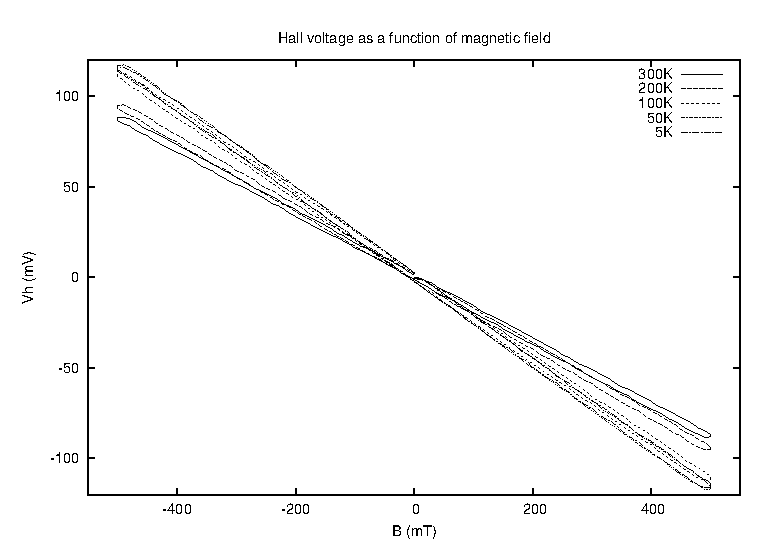
\includegraphics[width=0.45\textwidth]{tension_hall_fonction_champ.eps}
\caption{Hall voltage magnetic field response for different temperatures}
\label{fig:hall_champ}
\end{figure}

\begin{figure}[h]
\centering
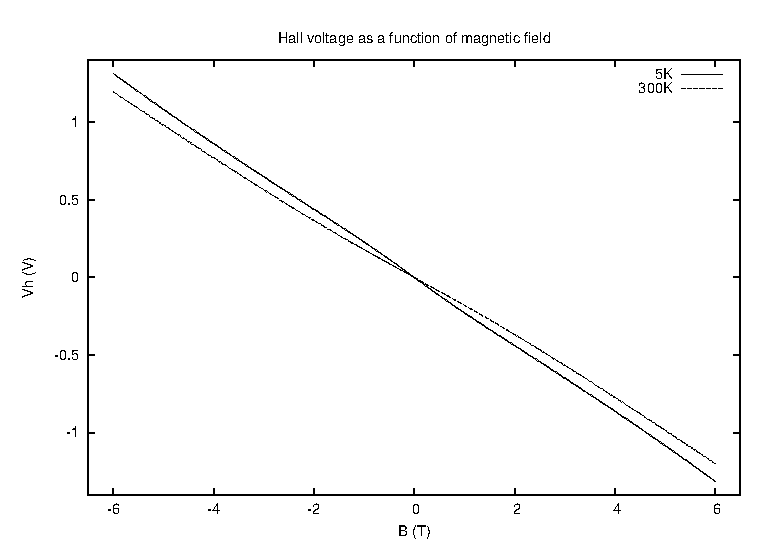
\includegraphics[width=0.45\textwidth]{tension_hall_fonction_champ_6T.eps}
\caption{Hall voltage response to a strong magnetic field}
\label{fig:hall_champ_6}
\end{figure}


%\subsubsection{Linear response}




\subsubsection{On the magnetic field in the cube}

We worked on the characterization of the magnetic field produced by the cube. The cube consists of eight induction coils, each one positioned at a vertex. By injecting current in those inductors a relatively high magnetic field (0.2 Tesla) is obtained in the center of the cube. The cube was further characterized in homogeneity and in current dependence.


%\subsubsection{Linear response}

First, the linear response of the field to the applied current was measured. The eight induction coils were connected in series in order to obtain a vertical magnetic field along the z-axis at maximum intensity. To measure the field created we used two different devices, the Gauss Meter KOSHAVA 5 and the previously discussed Hall bar sensor. A bipolar operational amplifier from Kepco ($\pm$ 36V, $\pm$ 6A) was used as the current source. It was able to provide a 3A current in the series connection of the coils. \figurename \ref{fig:linear_gauss} shows the vertical magnetic field as a function of current. These measurements were performed with the Gauss Meter from KOSHAVA.

Knowing the linear response measured with the commercial Gauss Meter, we conducted the same experiment using the Hall bar sensor to measure the intensity of the magnetic field. The results are shown on \figurename \ref{fig:linear_hall_20}. In order to get a good signal we had to make the measurements several times; the results presented are averaged over 20 points. This signal distortion meant that the commercial Gauss Meter was more useful in the measuring the magnetic field.

Second of all, the homogeneity of the field was studied. By controlling the movement of the Gauss Meter in each directions using verniers, we tried to draw a map of the field in the cube. At a fixed high, the Gauss Meter was moved on the two directions $x$ and $y$ by half a millimeter steps. We also measured the decrease of magnetic field norm at a fixed $(x,y)$ while changing the z-position. During both these experiments the inductors were still connected in series with a maximum current.





\begin{figure}[h]
\centering
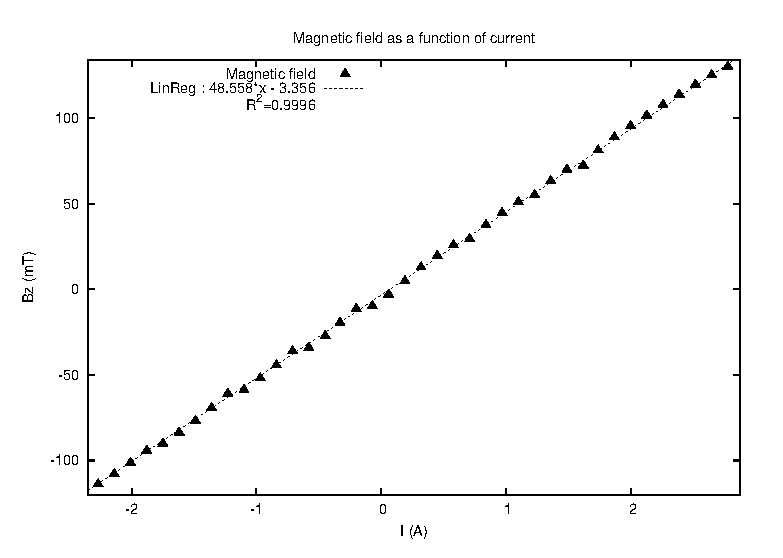
\includegraphics[width=0.45\textwidth]{champ_fonction_courant.eps}
\caption{The magnetic field as a function of current, measurements performed with the Gauss Meter}
\label{fig:linear_gauss}
\end{figure}



\begin{figure}[h]
\centering
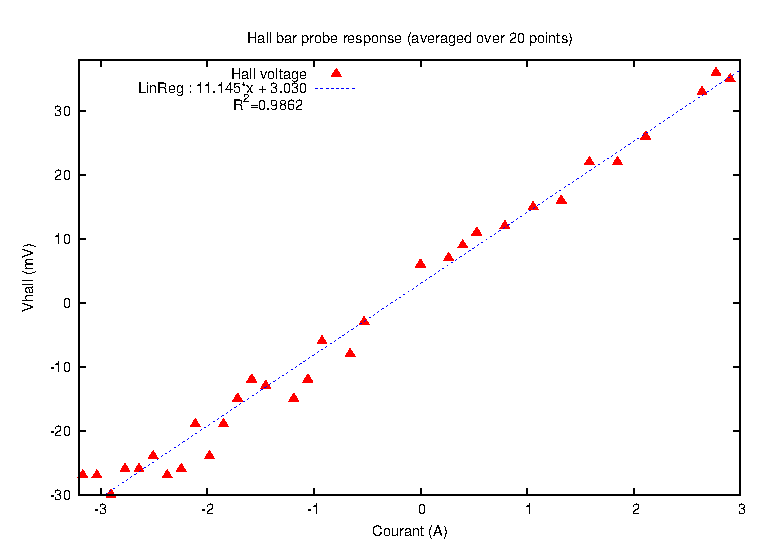
\includegraphics[width=0.45\textwidth]{rampe_courant_20.eps}
\caption{The magnetic field as a function of current, measurements performed with the Hall bar sensor}
\label{fig:linear_hall_20}
\end{figure}

\begin{figure}[h]
\centering
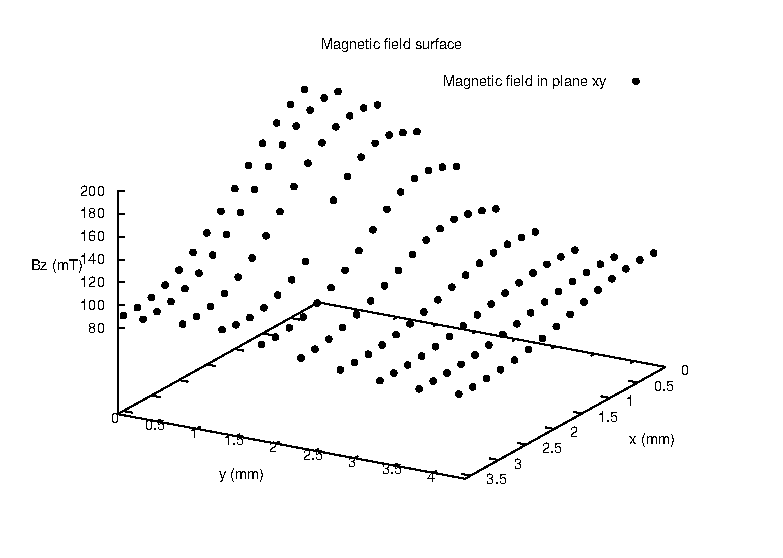
\includegraphics[width=0.45\textwidth]{cartographie_champ.eps}
\caption{A three-dimensional map of the magnetic field, created using the Gauss Meter}
\label{fig:map}
\end{figure}

\begin{figure}[h]
\centering
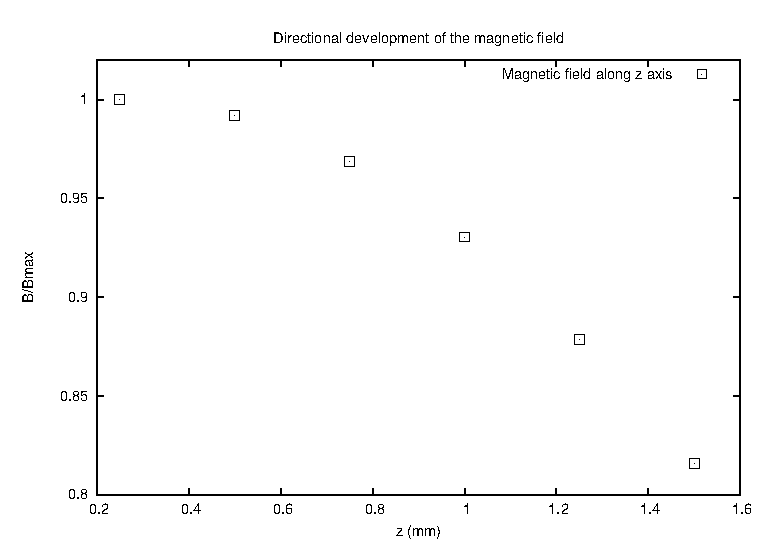
\includegraphics[width=0.45\textwidth]{cartographie_champ_z.eps}
\caption{Vertical homogeneity of the field}
\label{fig:homo_z}
\end{figure}

\subsection{Discussion}

\subsubsection{About the Hall bar sensor}

The \figurename \ref{fig:hall_champ} shows that the response of the Hall bar sensor to a magnetic field is linear through a large range of temperature. Since the slope depends on temperature,the Hall voltage at a given magnetic field can vary from 20mV. That tells us that the sensor may be useful to perform measurement but it has to be used carefully if placed directly in the cryostat.

Looking at \figurename \ref{fig:linear_hall_20} we see that (even though the measures were averaged over 20 points) the signal is not as good as the one we get with the Gauss Meter. Many things can explain this phenomena. First the Hall signal is very low and the input card reached its limit while measuring the signal. The Hall sensor was powered with a 1mA current and as stated in \cite{toshiba} it can be powered with currents up to 5mA. The lack of functioning control electronics also deteriorated the performance of the Hall bar sensor. 

\subsubsection{The magnetic field inside the cube}

As shown in \figurename \ref{fig:map} we were able to draw a map of the magnetic field norm in the center of the cube. This shows that it is homogeneous, at least at short range. Additionally, \figurename \ref{fig:homo_z} allows us to notice the homogeneity quantitatively. We see that a 5\% variation of the field appears in less than one millimeter, which is quite short considering the volume of the center of the cube to be at least $1\mathrm{cm^3}$.

The homogeneity of the field may be improved by taking the following measures. The coils are wrapped around cores, and it is possible to adjust the distances between the cores. A short distance between the cores will maximize the norm of the magnetic field, whereas a long distance will decrease it while improving homogeneity. Experiments varying the distances between the cores should be performed in order to see the qualitative effect on the homogeneity of the field. 

\section{Conclusion}

Several of our original objectives were meet. We were able to characterize the magnetic field created in the cube; software was developed to allow us to do this directly through a computer. This will allow for more accurate experimentation using the cube in the future. The software allows control of the cube's magnetic field, but would need to be further developed to allow for temperature control in the sample chamber, as well as more complete controls of the magnetic field.

The electronics necessary to use the Toshiba Hall bar as a magnetic field sensor are designed, although they will need to be fabricated again to be usable. This may allow the measurement of the magnetic field in the cube to be further improved.

Lastly, allow the cryostat was designed, the construction was not finished until after our project was over. We were never able to test our entire set-up together. The next natural step is to set up the cryostat, and using the computer controls, test the devices with a magneto-optical microscope.

\begin{figure}[h]
\centering
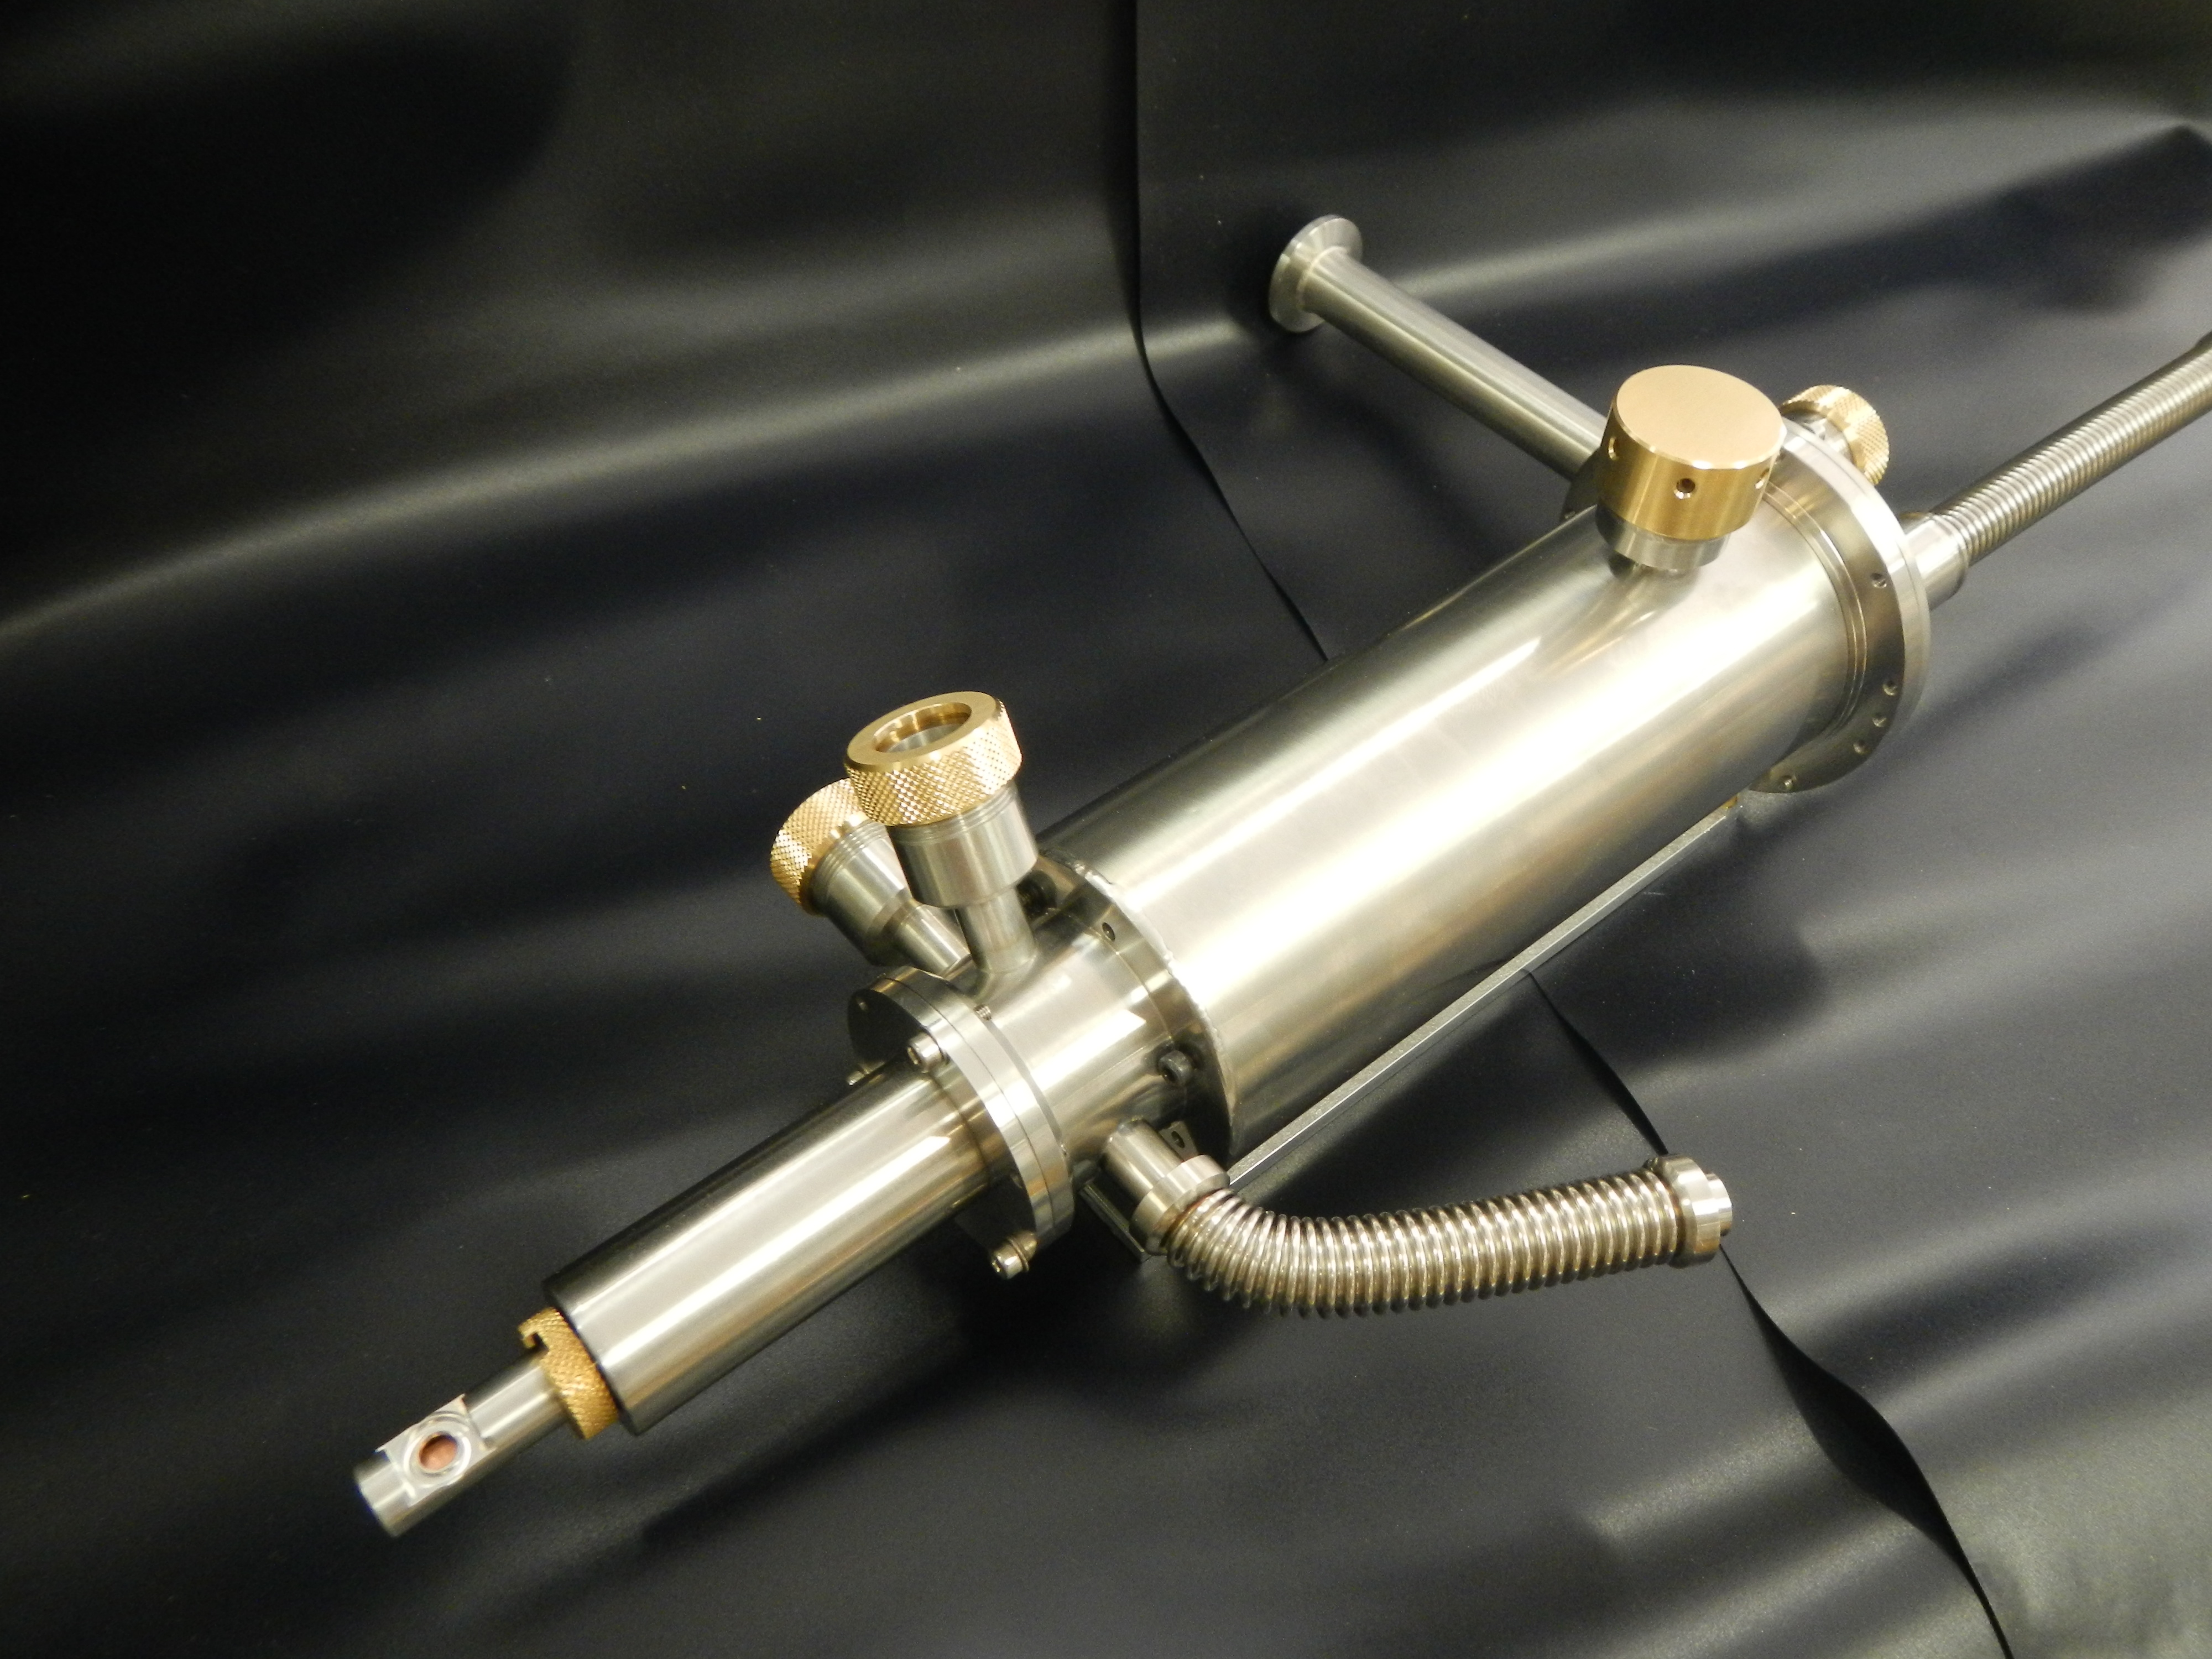
\includegraphics[width=0.45\textwidth]{cryostat1}
\caption{An image of the completed cryostat, which we unfortunately were never able to use}
\label{fig:cryostat1}
\end{figure}


% if have a single appendix:
%\appendix[Proof of the Zonklar Equations]
% or
%\appendix  % for no appendix heading
% do not use \section anymore after \appendix, only \section*
% is possibly needed

% use appendices with more than one appendix
% then use \section to start each appendix
% you must declare a \section before using any
% \subsection or using \label (\appendices by itself
% starts a section numbered zero.)
%


%\appendices
%\section{Proof of the First Zonklar Equation}
%Appendix one text goes here.

\appendix[Directional control of the magnetic field]\label{sec:app}

\section*{General case}

The three-dimensional magnetic field in the cube is created by four pairs of inductors. Assuming we have one current source for each pair of inductors, the magnetic field in the center of the cube is the sum of four vectors. Thus there is an infinite number of current combinaisons creating the same magnetic field (wich has three dimensions).

Let $ABCDEFGH$ be the cube (with $A(0,0,0)$ and $E(0,0,1)$). $ABCD$ is the bottom square face and $EFGH$ the top square face. Our four current sources allows us to create four magnetic fields in the center
\begin{IEEEeqnarray}{rCl} 
\mathbf{B_1} &=& \alpha \mathbf{AG}\IEEEyesnumber\IEEEyessubnumber\\
\mathbf{B_2} &=& \beta \mathbf{CE}\IEEEyessubnumber\\
\mathbf{B_3} &=& \gamma \mathbf{BH}\IEEEyessubnumber\\
\noalign{\noindent and\vspace{\jot}}
\mathbf{B_4} &=& \delta \mathbf{DF}\IEEEyessubnumber
\end{IEEEeqnarray}

We assume that the current flowing through the pairs of inductors is proportional to the magnetic field created, and that the magnetic field has a diagonal direction. We want to know how to choose $\alpha$, $\beta$, $\gamma$ and $\delta$ in order to get a magnetic field $\mathbf{B}$ with $x$, $y$, and $z$ as components. In the center of the cube the magnetic field is
\begin{equation} 
\label{eqn_B} 
\mathbf{B} = \sum\limits_{i=1}^{4} \mathbf{B_i} 
\end{equation}

We get a three-equations linear system wich has one degree of liberty. 
\begin{IEEEeqnarray}{rCl}
\label{sys_2} 
\beta &=& \alpha - \frac{x+y}{2}\IEEEyesnumber\IEEEyessubnumber\\
\gamma &=& \frac{y+z}{2} - \alpha\IEEEyessubnumber\\
\noalign{\noindent and\vspace{\jot}}
\delta &=& \frac{x+z}{2} - \alpha\IEEEyessubnumber
\end{IEEEeqnarray}



Thus we need another equation in order to have a linear system with a unique solution. For instance we can choose to minimize the Joule heating that is proportional to
\begin{equation} 
\label{eqn_P} 
P^2 = \alpha^2 + \beta^2 + \gamma^2 + \delta^2
\end{equation}

Taking the derivative of \ref{eqn_P} and equalizing it to zero we get a new equation
\begin{equation} 
\label{eqn_4} 
4 \alpha - \left(x + y + z\right) = 0
\end{equation}

The four-equation linear system we get with \ref{sys_2} and \ref{eqn_4} has a unique solution, wich is
\begin{IEEEeqnarray}{rCl} 
\alpha &=& \frac{1}{4} \left(x + y +z \right)\IEEEyesnumber\IEEEyessubnumber\\
\beta &=& \frac{1}{4} \left(-x - y +z \right)\IEEEyessubnumber\\
\gamma &=& \frac{1}{4} \left(-x + y +z \right)\IEEEyessubnumber\\
\noalign{\noindent and\vspace{\jot}}
\delta &=& \frac{1}{4} \left(x - y +z \right)\IEEEyessubnumber
\end{IEEEeqnarray}

\section*{Rotating magnetic field}

Using the calculations above we can generate a rotating magnetic field in the plane $xz$, with two current sources able to deliver sine currents. The currents are given by the following equations
\begin{IEEEeqnarray}{rCl} 
\alpha &=& \frac{1}{4} \left(\cos(\omega t) + \sin(\omega t) \right)\IEEEyesnumber\IEEEyessubnumber\\
\beta &=& \frac{1}{4} \left(- \cos(\omega t) + \sin(\omega t) \right)\IEEEyessubnumber\\
\gamma &=& \beta \IEEEyessubnumber\\
\noalign{\noindent and\vspace{\jot}}
\delta &=& \alpha \IEEEyessubnumber
\end{IEEEeqnarray}

Then the total magnetic field will be
\begin{equation} 
\label{eqn_B2} 
\mathbf{B} = \cos(\omega t) \mathbf{e_x} + \sin(\omega t) \mathbf{e_z}
\end{equation}

% you can choose not to have a title for an appendix
% if you want by leaving the argument blank
%\section{}
%Appendix two text goes here.


% use section* for acknowledgement
\section*{Acknowledgment}


The authors would like to thank supervisors Pierre Mohlo and Laurent Ranno of the Néel Institute, who made this project possible, as well as Didier Dufeu who designed the cryostat, and Daniel Lepoittevin who aided in the conception of the electronics for the Hall bar sensor.


% Can use something like this to put references on a page
% by themselves when using endfloat and the captionsoff option.
\ifCLASSOPTIONcaptionsoff
  \newpage
\fi



% trigger a \newpage just before the given reference
% number - used to balance the columns on the last page
% adjust value as needed - may need to be readjusted if
% the document is modified later
%\IEEEtriggeratref{8}
% The "triggered" command can be changed if desired:
%\IEEEtriggercmd{\enlargethispage{-5in}}

% references section

% can use a bibliography generated by BibTeX as a .bbl file
% BibTeX documentation can be easily obtained at:
% http://www.ctan.org/tex-archive/biblio/bibtex/contrib/doc/
% The IEEEtran BibTeX style support page is at:
% http://www.michaelshell.org/tex/ieeetran/bibtex/



\bibliographystyle{IEEEtran}
% argument is your BibTeX string definitions and bibliography database(s)
\bibliography{references}
%
% <OR> manually copy in the resultant .bbl file
% set second argument of \begin to the number of references
% (used to reserve space for the reference number labels box)

%\begin{thebibliography}{1}

%\bibitem{IEEEhowto:kopka}
%H.~Kopka and P.~W. Daly, \emph{A Guide to \LaTeX}, 3rd~ed.\hskip 1em plus
 % 0.5em minus 0.4em\relax Harlow, England: Addison-Wesley, 1999.

%\end{thebibliography}

% biography section
% 
% If you have an EPS/PDF photo (graphicx package needed) extra braces are
% needed around the contents of the optional argument to biography to prevent
% the LaTeX parser from getting confused when it sees the complicated
% \includegraphics command within an optional argument. (You could create
% your own custom macro containing the \includegraphics command to make things
% simpler here.)
%\begin{biography}[{\includegraphics[width=1in,height=1.25in,clip,keepaspectratio]{mshell}}]{Michael Shell}
% or if you just want to reserve a space for a photo:

%\begin{IEEEbiography}{Michael Shell}
%Biography text here.
%\end{IEEEbiography}

% if you will not have a photo at all:
%\begin{IEEEbiographynophoto}{John Doe}
%Biography text here.
%\end{IEEEbiographynophoto}

% insert where needed to balance the two columns on the last page with
% biographies
%\newpage

%\begin{IEEEbiographynophoto}{Jane Doe}
%Biography text here.
%\end{IEEEbiographynophoto}

% You can push biographies down or up by placing
% a \vfill before or after them. The appropriate
% use of \vfill depends on what kind of text is
% on the last page and whether or not the columns
% are being equalized.

%\vfill

% Can be used to pull up biographies so that the bottom of the last one
% is flush with the other column.
%\enlargethispage{-5in}



% that's all folks
\end{document}


